\documentclass{mcmthesis}
\mcmsetup{tcn = 1901923, problem = A, sheet = true, titleinsheet = true, keywordsinsheet = false, titlepage = false, abstract = false}
\usepackage{palatino}
\newcommand{\upcite}[1]{\textsuperscript{\textsuperscript{\cite{#1}}}}

\title{Ecological Strategy of Targaryens': How to Support Three Dragons?}
\date{\today}
\begin{document}
\begin{abstract}
In the series of novels \textit{A Song of Ice and Fire} by George R.R. Martin and the television series adapted from it, Deanerys Targaryen keeps three dragons. These dragons have quick growth rate and, therefore, have incredible impact on the local ecosystem. We establish a model of the dragons and discussion the interaction between the dragon and the ecosystem.

First, we analyse the dragon’s activity and interaction with ecosystem. We start building models of dragon’s energy consuming to describe its daily activities. We use existed activity models to reasonably predict dragon’s energy consumption. We use mammals’ metabolism model to describe dragon’s metabolism. After that, we build dragon’s flight model depending on birds' flight mechanism. Considering the abundance of research on mammals' walking mechanism, we use mammals’ walking model to describe dragon’s energy consumption for walk.We use dimensional method to estimate the power of fire breath. We create models to predict the pressure from dragons on ecosystem and community and find out that dragons have huge impact on local ecosystem. We create a model to describe the relationship among the energy assimilated by the dragon, the energy for growth and the energy for other daily activities.

We use 2D modeling technique and logistic model to simulate dragon’s growth model in different temperature and region and provide some rules between the variables.

Our further discussion focused on the dynamic change of dragon’s weight in different temperature and different biosystem.
\begin{keywords}
keyword1; keyword2
\end{keywords}
\end{abstract}
\maketitle

\tableofcontents

\newpage

\section{Introduction}

%Here is an example of itemize.
%\begin{itemize}
%\item minimizes the discomfort to the hands, or
%\item maximizes the outgoing velocity of the ball.
%\end{itemize}

%Here is an\upcite{knuth1984texbook} example\upcite{lamport1994latex} of\upcite{latexopensourcehouse} cite\upcite{latexopensourcehouse1}.

%Here are examples of Theorem, Lemma and proof.
%\begin{Theorem} \label{Label of lemma}
%Please write theorem here.
%\end{Theorem}
%\begin{Lemma} \label{Label of lemma}
%Please write lemma here.
%\end{Lemma}
%\begin{proof}
%The proof of theorem.
%\end{proof}

\subsection{Background}
Giant body, fire-breathing skills, durable flying ability and strong defense, in A song of Ice and Fire by R.T.Martin, Deanerys Targaryen’s three dragons have all these magical abilities. Now, assume these three dragons come to live today. So in the real world, the dragons grow from about $10$ kg to $40\sim50$ kg after the first year of their hatch. Their growth are influenced by the living condition. If the living condition is appropriate, they can keep growing throughout their lifetime. The fast growing rate of dragon also stresses the ecosystem. Therefore, we are going to explore the dragon’s characteristics, behavior, and its interaction with ecosystem as well, which will determine the energy requirement and growth limitation of dragon, the influence of the dragon to the ecosystem, the dragon’s daily performance and its energy consumption. Further, we will research the impact of different environments on dragon. 



\subsection{Our Work}
Our work consist of mainly four steps.

\begin{itemize} 
\item \textbf{Establish a model of the dragons' interaction with the environment.} To specify the dragon’s image, we add several reasonable assumptions about its biological feature and behavior. Based on these assumptions, we build a model to calculate dragons' energy consumption and weight growth and its impact on the local ecosystem.
\item \textbf{Discussion about different scenario and sensitivity analysis.} Using model build in former two steps, we investigate dragon's energy consumption growth and impact on the environment in different climate. We also conduct necessary sensitivity analysis.
\item \textbf{Suggestion letter to R.T.Martin.} We draft a letter to the fictional novel author, to provide suggestion to make the dragon more realistic in terms of ecology according to our study.
\end{itemize}

\section{Terminologies and Notations}

\subsection{Terminologies}
Here are some biological and ecological terminologies that we will use in the following sections:
\begin{itemize}
\item[\textbf{Endotherm}] also known as warm-blooded animal, the kind of animal that can maintain its body temperature constant, including mammals and birds;
\item[\textbf{Carnivore}] the kind of animal that only feed on meat;
\item[\textbf{Basal metabolism rate}] the rate of energy expenditure per unit time by endothermic animals at rest.
\end{itemize}
\subsection{Notations}
\begin{table}[h]
\centering
\caption{Main Variables}
\label{Variables}
\begin{tabular}{cp{10cm}c}
\toprule
Symbols & Definitions & Units\\
\midrule
$A$ & the energy assimilated by one dragon in one day & kJ/day\\
$G$ & one dragon's energy consumption for growth in one day & kJ/day\\
$R$ & one dragon's energy consumption for all other activities except growth in one day & kJ/day\\
$W(t)$ & one dragon's weight at day $t$ & kg\\
$\sigma$ & dragon body energy density --- the average energy stored in unit weight of the dragon & kJ/kg\\
$P_i$ & consumption power for activity $i$ & kJ/h\\
$t_i$ & hours for activity i in one day & h/day\\
$E_{\text{fire}}$ & energy consumption for breathing fire each time & kJ\\
$m$ & times that one dragon breathe fire in one day & kJ\\
$v_{walk}$ & the dragon's walking velocity & m/s\\
$v_{fly}$ & the dragon's flying velocity & m/s\\

\bottomrule
\end{tabular}
\end{table}

\section{Assumptions and Justification}
In fact, dragon is only a kind of fictional creature. To specify the image of dragon, we make the following assumption according to some plots in Martin's novel and features of similar animals, like lizards and birds:
\begin{itemize}
\item \textbf{Dragon is a kind of endotherm.} The wings on dragon's back make it like a giant bird in shape, and birds are known as typical endotherm. Besides, in Martin's novel and adapted television series, dragons have fought both near King's land (warm region) and beyond the Wall (cold region). Swift action in fight and good adaption to different environment temperature are usually the features of endotherm.
\item \textbf{Dragon is a kind of carnivore.} There is no record of dragon eating vegetables In Martin's novel.
\item \textbf{Dragons have two locomotive patterns: walk for short distance and fly for long distance. They can also breathe fire.}
\item \textbf{The three dragons are totally the same for simplicity.} So we only analyze one dragon and talk about the total impact of three dragon at the conclusion.
\end{itemize}
A few assumptions will be added at the proper place of the following article.

\section{Model of Individual Dragon}
Based on the assumptions proposed in last section, we establish an energy consumption and growth model for one single dragon in this section. According to theory of energy ecology\upcite{lu1987energy}, we divide the energy assimilated by the dragon every day into two parts. The dragon uses one part of the assimilated energy for growth, the other for other activities except growth.
\begin{equation}
\label{A}
A=G+R
\end{equation}
where \begin{itemize}
\item $A$ --- the energy assimilated by the dragon
\item $G$ --- the energy for growth
\item $R$ --- the energy for other activity
\end{itemize}

In next two subsections, we will formulate the function of each part of the equation above and find the relationship between the impact on the ecosystem and the assimilated energy or energy used for growth.

\subsection{Energy for Activities Except growth}

To calculate the energy one dragon consumed in daily life, we identify the four typical activities of dragon: rest, walking, flying and breathing fire. The energy a dragon consumes in one single day is the sum of product of time proportion in one day and power of energy consumption for each activity.
\begin{equation}
\label{R}
R=P_{\text{rest}}t_{\text{rest}}+P_{\text{walk}}t_{\text{walk}}+P_{\text{fly}}t_{\text{fly}}+mE_{\text{fire}}
\end{equation} 
where\begin{itemize}
\item $R$ --- the energy used for all life activities except growth in one day
\item $P_i$ --- the consumption power of activity $i$
\item $t_i$ --- lasting times of activity $i$ in one day
\item $m$ --- the times that the dragon breathes fire in one day
\item $E_{\text{fire}}$ --- the energy used for breathing fire each time
\end{itemize}

\textbf{Power of Rest}~~As we assumed before, the dragon is a kind of endotherm, like mammals and birds, so the basal metabolism rate of the dragon should be similar to a equally-weighted mammal or bird. Because of this, we use the empirical basal metabolism rate formula of mammals and birds\upcite{kolokotrones2010curvature}
\begin{equation}
\label{Prest}
P_{\text{rest}}=10^{[\beta_0+\beta_1\log_{10}M+\beta_2(\log_{10}M)^2+\beta_T/T]}
\end{equation}
where the constants $\beta_0=14.0149$, $\beta_1=0.5371$, $\beta_2=0.0294$, $\beta_T=-4799.0$, to calculate the consumption power of dragon in rest.

\textbf{Power for Walking}~~Taylor's article\upcite{taylor1982energetics} provides us with an empirical power function of animal's walking on flat ground
\begin{equation}
\label{Pwalk}
P_{walk}=38.52W^{0.684}\cdot v_{\text{walk}}+21.708W^{0.697}
\end{equation}
where\begin{itemize}
\item $P_{\text{walk}}$ --- power of energy consumption when dragon is creeping
\item $W$ --- weight of dragon
\item $v_{\text{walk}}$ --- creep velocity
\end{itemize}

\textbf{Power of Fly}~~Considering that dragon’s flight is similar to birds', it is reasonable to calculate dragon’s energy consumption with birds' equation. In the article \textit{Bird Metabolism During Flight : Evaluation of a Theory}\upcite{tucker1973bird}, Vance A. Tucker used least-square fitting techniques to derive birds' power consumption during flight
\begin{equation}
\label{Pfly}
P_{\text{fly}}=0.587W^{0.80}\cdot v_{\text{fly}}
\end{equation}
where\begin{itemize}
\item $P_{\text{fly}}$ --- the total energy consumption when flying
\item $W$ --- the weight of the flying animal
\item $v_{\text{fly}}$ --- the flying velocity
\end{itemize}

\textbf{Fire breathing}~~It is hard and unnecessary to give scientific explanation of dragon's fire breathing. We just skip its detailed mechanism, like the fuel and method of ignition. We use dimensional method to find the relationship between the total energy of each spray of fire and dragon’s weight.

To find determine the relationship, we have following local assumptions for fire breathing:
\begin{itemize}
\item the fire was sprayed from the dragon's throat. During fire breathing the energy flux density, $\mu$, at dragon's throat is constant.
\item the lasting time for each spray of fire, $t$, is the same
\end{itemize}

As we defined before, the energy flux density is the amount of energy flowing through a unit area during unit time, so the energy formula of each spray of fire is
\begin{equation}
\label{fire energy formula}
E_{\text{fire}}=\mu\cdot{S}\cdot t
\end{equation}
where\begin{itemize}
\item $\mu$ --- the energy flux density at dragon's throat (a constant value as we assumed before);
\item $S$ --- the cross-sectional area of dragon's throat as it is regard as a pipe.
\item $t$ --- the lasting time of each spray of fire (also a constant value);
\end{itemize}
We regard dragon's throat as a cylindrical pipe, we can write its cross-sectional area as
\begin{equation}
\label{S}
S=\frac{\pi d^2}{4}%~~\text{or}~~S\propto d^2
\end{equation}
where $d$ is the diameter of dragon's throat.

Like many other animals, the sizes of each body parts become larger proportionally during growth. According to dimensional analysis, the volume of dragon is proportional to cube of its length, so we have
\begin{equation}
\label{V}
V\propto d^3
\end{equation}

Besides, if the composition (like the percentage of protein, fat, water, etc) of dragon's body remains constant during its growth, the average density of dragon's body should also remain constant. If we define constant $\rho$ as its average density, we have
\begin{equation}
\label{W}
W\propto V
\end{equation}
Summarizing formula(\ref{fire energy formula}), (\ref{S}), (\ref{V}) and (\ref{W}), we find that the energy of fire breathing each time is proportional to weight's $(2/3)^{\text{th}}$ power
\begin{equation}
\label{Efire}
E_{\text{fire}}\propto W^{2/3}~~\text{or}~~E_{\text{fire}}=\alpha W^{2/3}
\end{equation}
where $\alpha$ is a constant that we are going to estimate next.

With equation(\ref{Efire}), given the energy consumption of fire breathing and weight at certain time, we can determine the coefficient $\alpha$. Recalling the story plot that a young dragon have cooked a small piece of meat with its fire\upcite{gameofthrones}, we estimate its weight as $10$ kg and the meat's as $0.1$ kg at that time. As a survey report shows, the water content in pork in market ranges from $58.0\%$ to $75.2\%$\upcite{zhang1993porkinvestigation}, so we set the water content in the meat as $60\%$. Regardless of the energy loss, the energy of the fire raised the meat's temperature from $20^{\circ}$C to $100^{\circ}$C and transfer third of the water into steam, so we estimate the energy consumption of a spray of fire is $76.368$ kJ and the $\alpha$ is $32.233 \text{kJ}/\text{m}^2$.

\subsection{Assimilated Energy: Model One}
As the assumption we proposed before, dragon is a kind of carnivore. All the energy assimilated by the dragon is from its prey. In the meantime, the dragon's predation. To understand how the energy assimilated by the dragon change, we need to understand how the scale of its prey change.We need to build a model of how the prey's population change under the predation of the dragon.
To simplify the problem, we first consider the situation without dragon. If we do not consider the constrain of natural resources on the dragon, then the net growth rate of the prey stay a constant all the time. This means the population always increase a constant percentage in unit time, so we have
\begin{equation}
\label{growth rate}
\frac{dx_1/dt}{x_1}=r_1
\end{equation}
where \begin{itemize}
\item $r_1$ --- the growth rate of the prey
\end{itemize}
We solve equation(\ref{growth rate}) and get an exponential growth function of the prey's population
\begin{equation}
x_1(t)=x_1(0)e^{r_1t}
\end{equation}
where \begin{itemize}
\item $x_1(0)$ --- the initial population of the prey
\end{itemize}
However, the exponential growth pattern will lead to explosive increase in a short time as shown in figure \ref{exponential growth plot} ,which is hardly seen in reality.
Here is an example of figure.
\begin{figure}[h]
\small
\centering
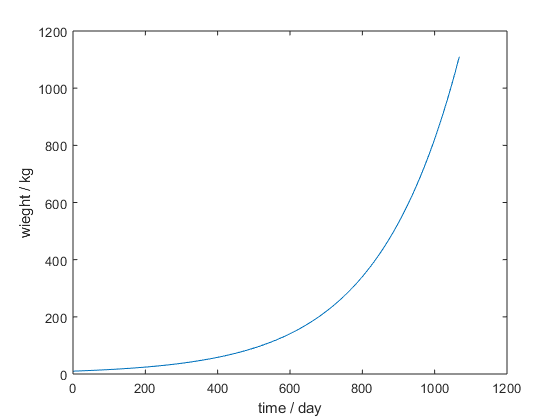
\includegraphics[width=12cm]{exponential}
\caption{The exponential growth pattern of population}\label{exponential growth plot}
\end{figure}
In fact, the population growth rate of most the creatures are constrained by various natural conditions. As the population approaches the upper limit, the constrain on the growth rate become greater. If we assume that the growth rate decreases linearly with population's increase,
\begin{equation}
r_1=r_{10}(1-\frac{x_1}{x_{1\max}})
\end{equation}
where \begin{itemize}
\item $r_{10}$ --- the growth rate of the prey when there is no constrain of natural condition
\item $x_{1\max}$ --- the balanced population of the prey
\end{itemize}
then we solve equation \ref{growth rate} and get
\begin{equation}
x_1(t)=\frac{x_{1\max}}{1+(\frac{x_{1\max}}{x_10}-1)e^{-rt}}
\end{equation}
In this way, the population can reach an upper limit as shown in figure \ref{logistic growth plot} which is more reasonable for the population in reality.
\begin{figure}[h]
\small
\centering
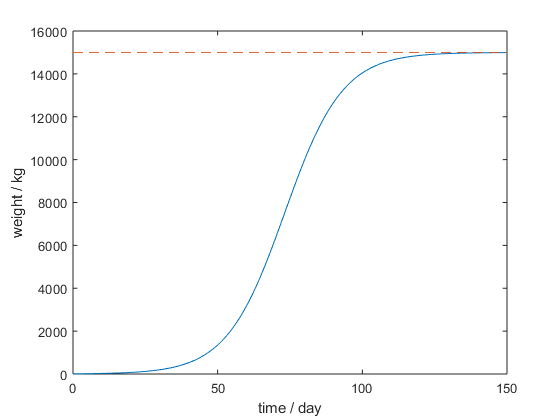
\includegraphics[width=12cm]{standard_logistic}
\caption{The logistic growth pattern of population}\label{logistic growth plot}
\end{figure}
Now we consider the situation with a predator's existence, the growth rate of the prey is also constrained by the population of the predator. According to\upcite{chen1988math}, we can write the growth rate of prey as
\begin{equation}
r=r_{10}(1-\frac{x_1}{x_{1\max}}-\frac{x_2}{x_{2\max}})
\end{equation}
so we have
\begin{equation}
\label{prey}	
\frac{dx_1/dt}{x_1}=r_{10}(1-\frac{x_1}{x_{1\max}}-\sigma_1\frac{x_2}{x_{2\max}})
\end{equation}
where\begin{itemize}
\item $x_2$ --- the population of the predator
\item $x_max$ --- the balanced population of predator
\item $\sigma_1$ --- a constant representing the extend of predator's threat on the growth rate of the population of prey
\end{itemize}
At the same time, the predator has population
\begin{equation}
\label{predator}
\frac{dx_2/dt}{x_2}=r_{20}(1+\sigma_2\frac{x_1}{x_{1\max}}-\frac{x_2}{x_{2\max}})
\end{equation}
where\begin{itemize}
\item $\sigma_2$ --- a constant representing the extend of prey's supporting for the growth rate of the population of prey
\end{itemize}
Here in our case, the predator is only one dragon, but according to the analysis above, we can still apply equation(\ref{prey}) to the prey's population while we regard the dragon's weight as the predator's population. Besides, we replace the item $-r_{20}\frac{x_2}{x_{2\max}}$ with $R/\rho$. The item $R/\rho$ represent the weight loss in unit time due to energy consumption for activities except growth, which just means the dragon's weight's threat on its growth rate. ($R$ --- energy consumption in unit time for activities except growth, $\rho$ --- energy density of dragon's body)
\begin{equation}
\left\{\begin{array}{ll}
\frac{dx_1/dt}{x_1}=r_{10}(1-\frac{x_1}{x_{1\max}}-\sigma_1\frac{W}{W_{\max}})\\
\frac{dW/dt}{W}=r_{20}(1+\sigma_2\frac{x_1}{x_{1\max}})-\frac{R}{\rho}
\end{array}\right.
\end{equation}
However, the sensitivity analysis on parameters $\sigma_1$ and $\sigma_2$ shows that the model is not very stable. In some case, the population and the weight of the dragon can reach a balanced state (shown in figure \ref{stable}) while in other case, thees two value end to be zeros (shown in figure \ref{unstable}, the ecosystem collapses). Besides, we find that the transfer threshold between the two kinds of result also varies with the value of parameters $r_{10}$ and $r_{20}$. However, these two parameter can only be estimated because there is not any reference data of them.
\begin{figure}[h]
\small
\centering
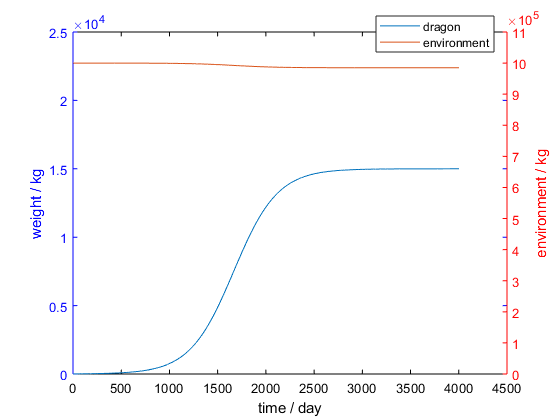
\includegraphics[width=10cm]{stable}
\caption{The population of the prey and the weight of the the dragon reach a balanced state($\sigma_1=6000$, $\sigma_2=0.1$)}\label{stable}
\end{figure}

\begin{figure}[h]
\small
\centering
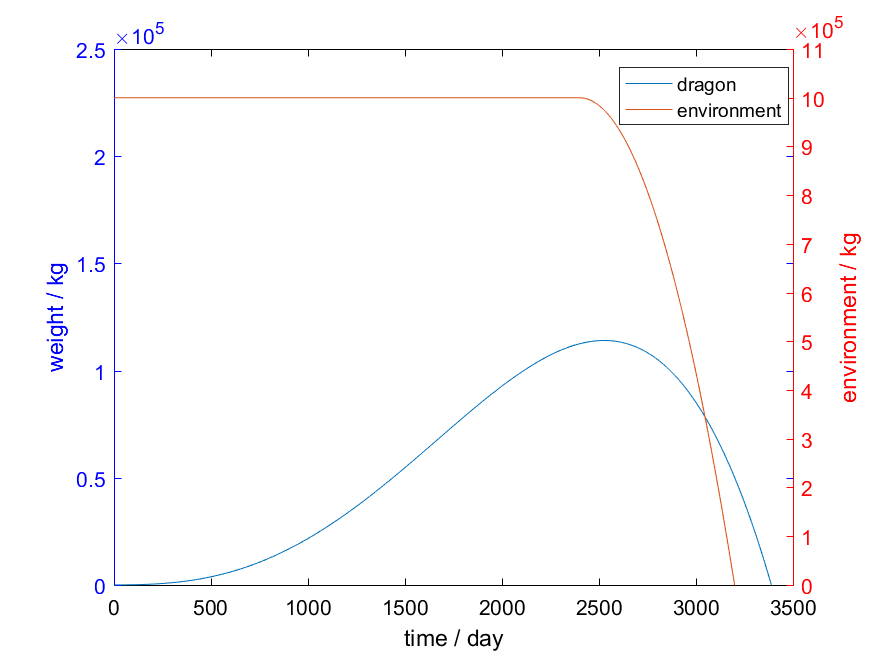
\includegraphics[width=10cm]{unstable}
\caption{The population of the prey and the weight of the the dragon end to be zeros ($\sigma_1=6100$, $\sigma_2=0.1$)}\label{unstable}
\end{figure}

\subsection{Assimilated Energy: Model Two}
To get rid of the instability of the former assimilated energy model, we establish a more simple model in this section. Since there is only one dragon with a much larger population of prey if there are enough area to support the dragon, the dragon's predation have limited impact on the population of the prey. In this case, the population of the prey will stay almost unchanged like figure \ref{stable}. Therefore, the food supply for the dragon will stay unchanged and the dragon weight growth is only constrained by its growing energy consumption for other activities except growth.

In this way, the dragon's weight growth will be very similar to the logistic pattern, so we use logistic function to represent its weight growth directly.

%We assume the growth rate of dragon's weight is constant. In other words, the dragon's weight gained in unit time is proportional to its weight, so we have
%\begin{equation}
%\label{differential equation of exponential growth}
%\frac{dW}{dt}=rW
%\end{equation}
%where\begin{itemize}
%\item $W$ --- the weight of the dragon
%\item $r$ --- the weight growth rate of the dragon, the percentage of weight gained in unite time
%\end{itemize}
%We solve the differential equation(\ref{differential equation of exponential growth}) and get an exponential growth function of dragon's weight,
%\begin{equation}
%\label{exponential growth}
%W(t)=W(0)e^{rt}
%\end{equation}
%If the dragon grows from $10$ kg to $50$ kg in the first year, then
%\begin{equation}
%W(t)=10\exp(\frac{t\ln5}{365})
%\end{equation}
%However, exponential growth curve in figure shows that 
%In fact, as a common sense of ecology, once (also almost always) there is constrain condition, most biological variables' growth rate will be constrained by  in logistic pattern rather than exponential pattern\upcite{haberman1998mathematical}. In this case, the weight growth rate of dragon is constrained by its weight in the following way
\begin{equation}
r=r_0(1-\frac{W}{W_m})
\end{equation}
where\begin{itemize}
\item $r_0$ --- the weight growth rate when growing without constrain
\item $W_m$ --- the maximum weight that a dragon can reach under constrain condition
\end{itemize}
Therefore, the weigh gained in unit time is
\begin{equation}
\label{logistic growth}
\frac{dW}{dt}=rW=r_0W(1-\frac{W}{W_m})
\end{equation}
We solve the differential equation(\ref{logistic growth}) and get the logistic growth equation for dragon's weight
\begin{equation}
W(t)=\frac{W_m}{1+(\frac{W_m}{W_0}-1)e^{-r_0t}}
\end{equation}
and the energy for weight growth in unit time is
\begin{equation}
\label{G}
G=\rho\frac{dW}{dt}
\end{equation}
where $\rho$ --- the energy density of the dragon's body.
Using equation (\ref{R}), (\ref{Prest}), (\ref{Pfly}), (\ref{Pwalk}), (\ref{Efire}), (\ref{G}), we get the final formula for dragon's assimilated energy
\begin{align}
A=&10^{[\beta_0+\beta_1\log_{10}M+\beta_2(\log_{10}M)^2+\beta_T/T]}t_{\text{rest}}\\&+(38.52W^{0.684}\cdot v_{\text{walk}}+21.708W^{0.697})t_{\text{walk}}\\
&+0.587W^{0.80}\cdot v_{\text{fly}}t_{\text{fly}}\\
&+\alpha mW^{2/3}\\
&+\rho r_0W(1-\frac{W}{W_m})
\end{align}
%\section{Discussion about different scenario and Sensitivity Analysis}
%\subsection{Discussion about the Dragon in Different R}
%In the last section, we build the energy consumption model of the dragon and its impact on the environment. In this subsection, we consider the situation when the dragon live in different region. The different climates make differences in mainly two aspects: different temperatures will cause different metabolism rates of the dragon and different climate will lead to different species and population (biomass) of the prey.
%
%As the assimilated energy of the predator (the dragon) is usually proportional to the energy flowing
%However, due to the limit of data, we can not conduct further calculation.

\section{Strengths and weaknesses}
\subsection{Strengths}
\begin{itemize}
\item \textbf{Using just a few variables.}\\
For example, when we calculate the assimilated energy, our model one described the dynamic relationship between ecosystem and dragon with just a few variables and model 2 used even fewer than model one to describe the relationship.
\item \textbf{Build solid connection between ecosystem and dragon’s energy consumption.}\\
By setting reasonable hypothesis and variables, we discovered the responsibly relationship between dragon’s energy consumption and ecosystem. We can predict dragons’ weight by some measurable statistics. It is a workable methodology investigate ecosystem’s internal interactions.
\end{itemize}

\subsection{Weakness}
\begin{itemize}
\item \textbf{Some empirical formula about dragon’s energy consumption may be not accurate.}\\
For example, the walking consumption power equation comes from articles studying walking mammals. Similar situations happened for the flying consumption power when the empirical formula is derived from the data of bird weighing less than 100kg. There is no existing theories for an animal like the dragon.
\item \textbf{We can only give the method to calculate the area needed to support the dragons but not the specific value.}\\
It is hard to get the data about biomass of different region in limit time, so  we can not calculate the specific values.
\end{itemize}

\section{Conclusion}
We provide a detailed analysis of dragon’s activity and interaction with ecosystem. We start building models of dragon’s energy consuming to describe its daily activities. First, we use existed activity models to reasonably predict dragon’s energy consumption.

We create models to predict the pressure from dragons on ecosystem and community and find out that dragons have huge impact on local ecosystem, a dragon consumes nearly two percent of energy in primary consumers. We also conclude that despite its tremendous consumption, dragons are not suitable for long distant flight.

We simulate dragon’s growth model in different temperature and region and provide some Find some rules between the variables.

\section{A Letter to George R.R. Martin}
Dear Mr.George:

Hello!

I’m a fan of your series of novels A song of Ice and Fire. The dragons in your book truly amazed me. While I was reading the books, I often imagined that the dragons might live in the modern society someday. Based on that idea, we made several assumptions and explored the dragon’s basic demand for life and its interaction with different environment. 
In our model, we refer to some real world animals’ energy consumption. Then we reach a conclusion that the dragons’ action in the novel is unscientific. The dragon’s energy reserve can never support it to take vigorous exercise like flying over thousands of kilometers in a day, but in the novel the dragon also needs to fight against enemies. And the fighting force may not be so strong as it is described in the novel. The dragon is so heavy that every movement of it expends much energy. Furthermore, in the TV series, the fire breathed out by the dragon can burn a group of soldiers to ashes. However the dragon can only roast a piece of meat when it is young. It is contradictory to the assumption that the energy flux density of fire stays the same. Considering the increase of weight, the dragon’s energy expenditure grows more dramatically. Therefore, the dragon depicted in the TV series is too heavy. To support three dragons is beyond the ecological as well as the  economical ability.

Yours,

Team 1901923


\addcontentsline{toc}{section}{Reference}
\bibliography{1901923.bib}
\bibliographystyle{unsrt}%{siam}%unsrt按引用先后排序

\end{document}